\documentclass[1p]{elsarticle_modified}
%\bibliographystyle{elsarticle-num}

%\usepackage[colorlinks]{hyperref}
%\usepackage{abbrmath_seonhwa} %\Abb, \Ascr, \Acal ,\Abf, \Afrak
\usepackage{amsfonts}
\usepackage{amssymb}
\usepackage{amsmath}
\usepackage{amsthm}
\usepackage{scalefnt}
\usepackage{amsbsy}
\usepackage{kotex}
\usepackage{caption}
\usepackage{subfig}
\usepackage{color}
\usepackage{graphicx}
\usepackage{xcolor} %% white, black, red, green, blue, cyan, magenta, yellow
\usepackage{float}
\usepackage{setspace}
\usepackage{hyperref}

\usepackage{tikz}
\usetikzlibrary{arrows}

\usepackage{multirow}
\usepackage{array} % fixed length table
\usepackage{hhline}

%%%%%%%%%%%%%%%%%%%%%
\makeatletter
\renewcommand*\env@matrix[1][\arraystretch]{%
	\edef\arraystretch{#1}%
	\hskip -\arraycolsep
	\let\@ifnextchar\new@ifnextchar
	\array{*\c@MaxMatrixCols c}}
\makeatother %https://tex.stackexchange.com/questions/14071/how-can-i-increase-the-line-spacing-in-a-matrix
%%%%%%%%%%%%%%%

\usepackage[normalem]{ulem}

\newcommand{\msout}[1]{\ifmmode\text{\sout{\ensuremath{#1}}}\else\sout{#1}\fi}
%SOURCE: \msout is \stkout macro in https://tex.stackexchange.com/questions/20609/strikeout-in-math-mode

\newcommand{\cancel}[1]{
	\ifmmode
	{\color{red}\msout{#1}}
	\else
	{\color{red}\sout{#1}}
	\fi
}

\newcommand{\add}[1]{
	{\color{blue}\uwave{#1}}
}

\newcommand{\replace}[2]{
	\ifmmode
	{\color{red}\msout{#1}}{\color{blue}\uwave{#2}}
	\else
	{\color{red}\sout{#1}}{\color{blue}\uwave{#2}}
	\fi
}

\newcommand{\Sol}{\mathcal{S}} %segment
\newcommand{\D}{D} %diagram
\newcommand{\A}{\mathcal{A}} %arc


%%%%%%%%%%%%%%%%%%%%%%%%%%%%%5 test

\def\sl{\operatorname{\textup{SL}}(2,\Cbb)}
\def\psl{\operatorname{\textup{PSL}}(2,\Cbb)}
\def\quan{\mkern 1mu \triangleright \mkern 1mu}

\theoremstyle{definition}
\newtheorem{thm}{Theorem}[section]
\newtheorem{prop}[thm]{Proposition}
\newtheorem{lem}[thm]{Lemma}
\newtheorem{ques}[thm]{Question}
\newtheorem{cor}[thm]{Corollary}
\newtheorem{defn}[thm]{Definition}
\newtheorem{exam}[thm]{Example}
\newtheorem{rmk}[thm]{Remark}
\newtheorem{alg}[thm]{Algorithm}

\newcommand{\I}{\sqrt{-1}}
\begin{document}

%\begin{frontmatter}
%
%\title{Boundary parabolic representations of knots up to 8 crossings}
%
%%% Group authors per affiliation:
%\author{Yunhi Cho} 
%\address{Department of Mathematics, University of Seoul, Seoul, Korea}
%\ead{yhcho@uos.ac.kr}
%
%
%\author{Seonhwa Kim} %\fnref{s_kim}}
%\address{Center for Geometry and Physics, Institute for Basic Science, Pohang, 37673, Korea}
%\ead{ryeona17@ibs.re.kr}
%
%\author{Hyuk Kim}
%\address{Department of Mathematical Sciences, Seoul National University, Seoul 08826, Korea}
%\ead{hyukkim@snu.ac.kr}
%
%\author{Seokbeom Yoon}
%\address{Department of Mathematical Sciences, Seoul National University, Seoul, 08826,  Korea}
%\ead{sbyoon15@snu.ac.kr}
%
%\begin{abstract}
%We find all boundary parabolic representation of knots up to 8 crossings.
%
%\end{abstract}
%\begin{keyword}
%    \MSC[2010] 57M25 
%\end{keyword}
%
%\end{frontmatter}

%\linenumbers
%\tableofcontents
%
\newcommand\colored[1]{\textcolor{white}{\rule[-0.35ex]{0.8em}{1.4ex}}\kern-0.8em\color{red} #1}%
%\newcommand\colored[1]{\textcolor{white}{ #1}\kern-2.17ex	\textcolor{white}{ #1}\kern-1.81ex	\textcolor{white}{ #1}\kern-2.15ex\color{red}#1	}

{\Large $\underline{12n_{0780}~(K12n_{0780})}$}

\setlength{\tabcolsep}{10pt}
\renewcommand{\arraystretch}{1.6}
\vspace{1cm}\begin{tabular}{m{100pt}>{\centering\arraybackslash}m{274pt}}
\multirow{5}{120pt}{
	\centering
	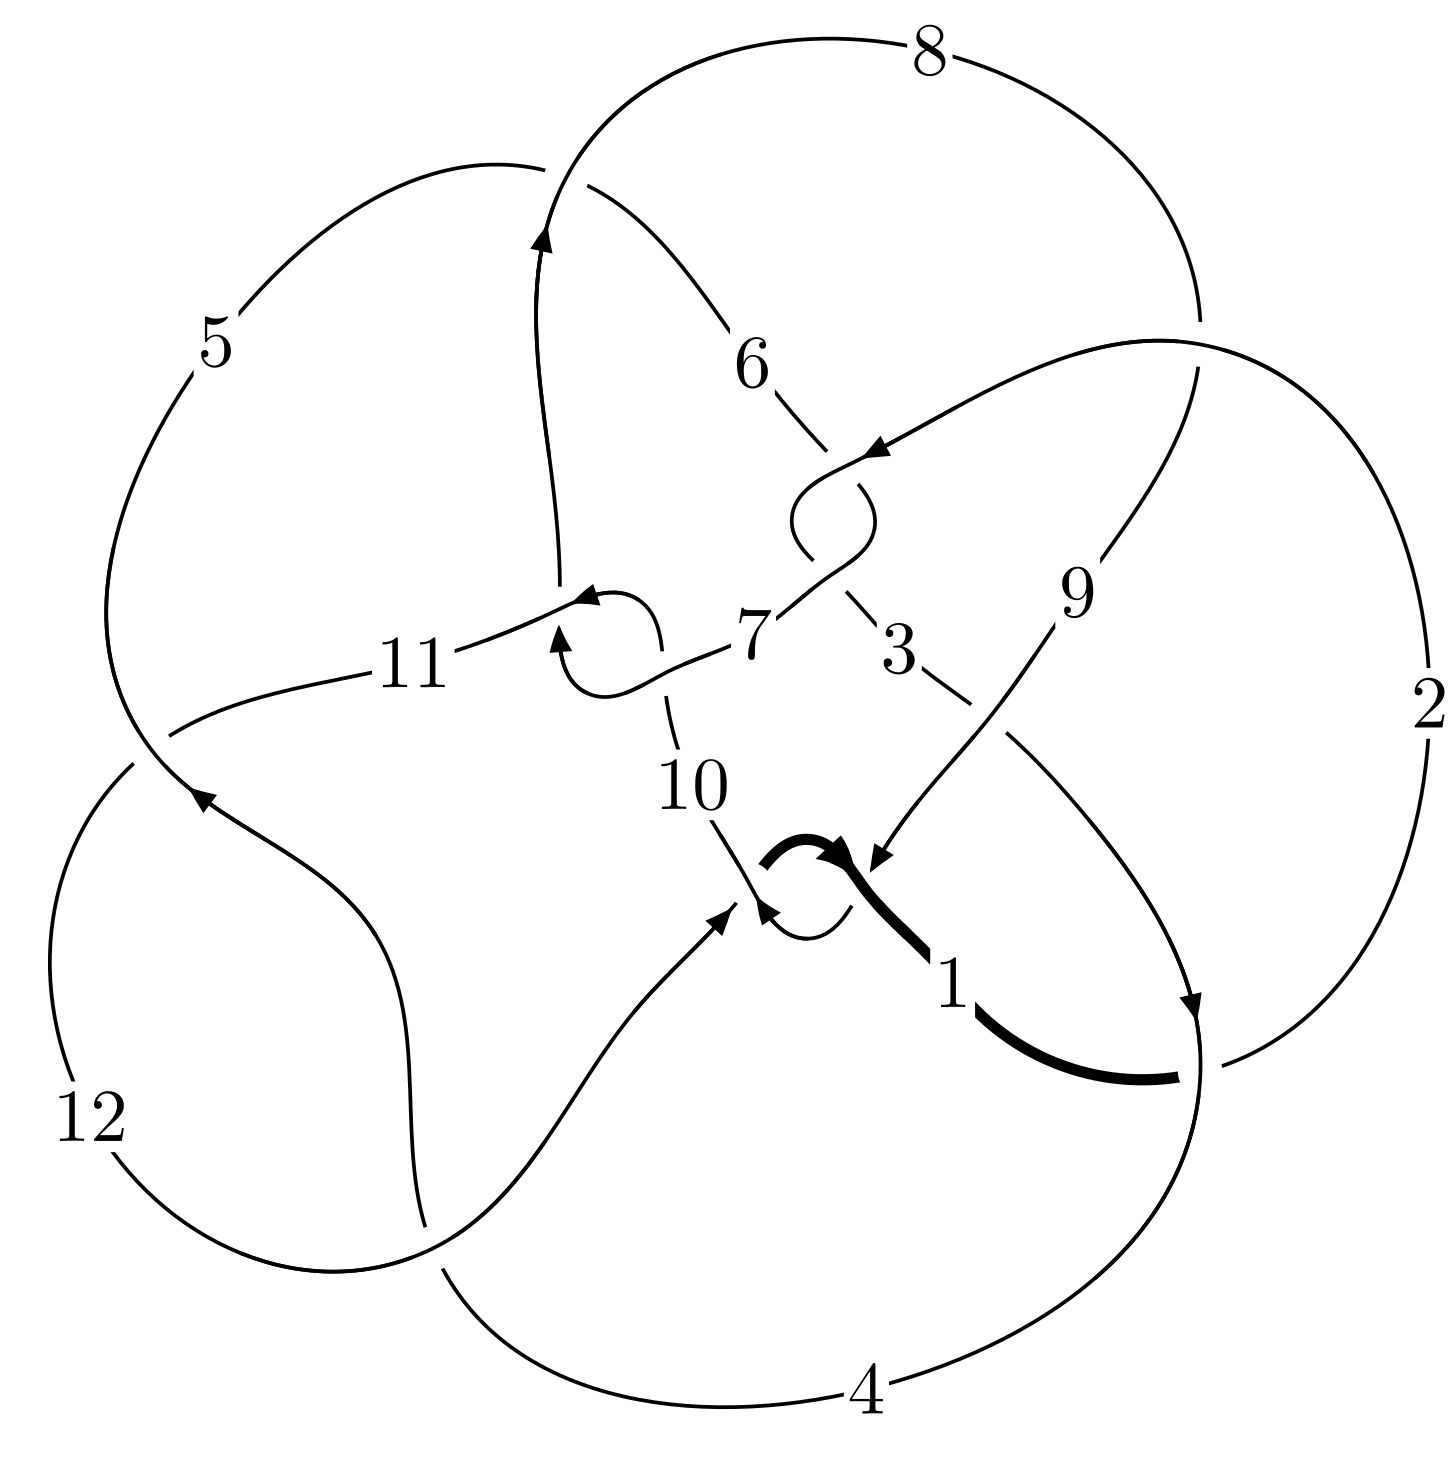
\includegraphics[width=112pt]{../../../GIT/diagram.site/Diagrams/png/2869_12n_0780.png}\\
\ \ \ A knot diagram\footnotemark}&
\allowdisplaybreaks
\textbf{Linearized knot diagam} \\
\cline{2-2}
 &
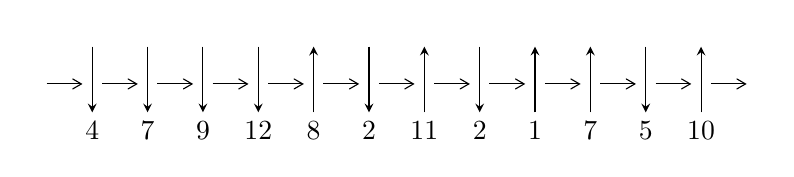
\begin{tikzpicture}[x=20pt, y=17pt]
	% nodes
	\node (C0) at (0, 0) {};
	\node (C1) at (1, 0) {};
	\node (C1U) at (1, +1) {};
	\node (C1D) at (1, -1) {4};

	\node (C2) at (2, 0) {};
	\node (C2U) at (2, +1) {};
	\node (C2D) at (2, -1) {7};

	\node (C3) at (3, 0) {};
	\node (C3U) at (3, +1) {};
	\node (C3D) at (3, -1) {9};

	\node (C4) at (4, 0) {};
	\node (C4U) at (4, +1) {};
	\node (C4D) at (4, -1) {12};

	\node (C5) at (5, 0) {};
	\node (C5U) at (5, +1) {};
	\node (C5D) at (5, -1) {8};

	\node (C6) at (6, 0) {};
	\node (C6U) at (6, +1) {};
	\node (C6D) at (6, -1) {2};

	\node (C7) at (7, 0) {};
	\node (C7U) at (7, +1) {};
	\node (C7D) at (7, -1) {11};

	\node (C8) at (8, 0) {};
	\node (C8U) at (8, +1) {};
	\node (C8D) at (8, -1) {2};

	\node (C9) at (9, 0) {};
	\node (C9U) at (9, +1) {};
	\node (C9D) at (9, -1) {1};

	\node (C10) at (10, 0) {};
	\node (C10U) at (10, +1) {};
	\node (C10D) at (10, -1) {7};

	\node (C11) at (11, 0) {};
	\node (C11U) at (11, +1) {};
	\node (C11D) at (11, -1) {5};

	\node (C12) at (12, 0) {};
	\node (C12U) at (12, +1) {};
	\node (C12D) at (12, -1) {10};
	\node (C13) at (13, 0) {};

	% arrows
	\draw[->,>={angle 60}]
	(C0) edge (C1) (C1) edge (C2) (C2) edge (C3) (C3) edge (C4) (C4) edge (C5) (C5) edge (C6) (C6) edge (C7) (C7) edge (C8) (C8) edge (C9) (C9) edge (C10) (C10) edge (C11) (C11) edge (C12) (C12) edge (C13) ;	\draw[->,>=stealth]
	(C1U) edge (C1D) (C2U) edge (C2D) (C3U) edge (C3D) (C4U) edge (C4D) (C5D) edge (C5U) (C6U) edge (C6D) (C7D) edge (C7U) (C8U) edge (C8D) (C9D) edge (C9U) (C10D) edge (C10U) (C11U) edge (C11D) (C12D) edge (C12U) ;
	\end{tikzpicture} \\
\hhline{~~} \\& 
\textbf{Solving Sequence} \\ \cline{2-2} 
 &
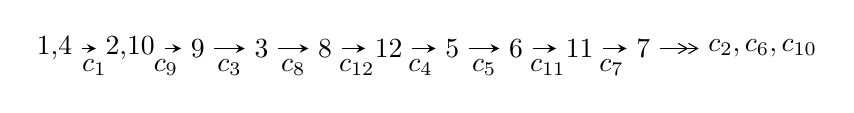
\begin{tikzpicture}[x=23pt, y=7pt]
	% node
	\node (A0) at (-1/8, 0) {1,4};
	\node (A1) at (17/16, 0) {2,10};
	\node (A2) at (17/8, 0) {9};
	\node (A3) at (25/8, 0) {3};
	\node (A4) at (33/8, 0) {8};
	\node (A5) at (41/8, 0) {12};
	\node (A6) at (49/8, 0) {5};
	\node (A7) at (57/8, 0) {6};
	\node (A8) at (65/8, 0) {11};
	\node (A9) at (73/8, 0) {7};
	\node (C1) at (1/2, -1) {$c_{1}$};
	\node (C2) at (13/8, -1) {$c_{9}$};
	\node (C3) at (21/8, -1) {$c_{3}$};
	\node (C4) at (29/8, -1) {$c_{8}$};
	\node (C5) at (37/8, -1) {$c_{12}$};
	\node (C6) at (45/8, -1) {$c_{4}$};
	\node (C7) at (53/8, -1) {$c_{5}$};
	\node (C8) at (61/8, -1) {$c_{11}$};
	\node (C9) at (69/8, -1) {$c_{7}$};
	\node (A10) at (11, 0) {$c_{2},c_{6},c_{10}$};

	% edge
	\draw[->,>=stealth]	
	(A0) edge (A1) (A1) edge (A2) (A2) edge (A3) (A3) edge (A4) (A4) edge (A5) (A5) edge (A6) (A6) edge (A7) (A7) edge (A8) (A8) edge (A9) ;
	\draw[->>,>={angle 60}]	
	(A9) edge (A10);
\end{tikzpicture} \\ 

\end{tabular} \\

\footnotetext{
The image of knot diagram is generated by the software ``\textbf{Draw programme}" developed by Andrew Bartholomew(\url{http://www.layer8.co.uk/maths/draw/index.htm\#Running-draw}), where we modified some parts for our purpose(\url{https://github.com/CATsTAILs/LinksPainter}).
}\phantom \\ \newline 
\centering \textbf{Ideals for irreducible components\footnotemark of $X_{\text{par}}$} 
 
\begin{align*}
I^u_{1}&=\langle 
2.42402\times10^{224} u^{66}+2.00218\times10^{225} u^{65}+\cdots+1.65127\times10^{226} b-1.54654\times10^{227},\\
\phantom{I^u_{1}}&\phantom{= \langle  }-8.95512\times10^{225} u^{66}-7.50188\times10^{226} u^{65}+\cdots+9.90762\times10^{226} a+5.44058\times10^{227},\\
\phantom{I^u_{1}}&\phantom{= \langle  }u^{67}+8 u^{66}+\cdots-598 u-48\rangle \\
I^u_{2}&=\langle 
-2.15444\times10^{23} u^{24}+2.41942\times10^{24} u^{23}+\cdots+2.49434\times10^{24} b+2.77494\times10^{24},\\
\phantom{I^u_{2}}&\phantom{= \langle  }-3.61629\times10^{24} u^{24}+3.77069\times10^{25} u^{23}+\cdots+1.74604\times10^{25} a+3.58327\times10^{24},\\
\phantom{I^u_{2}}&\phantom{= \langle  }u^{25}-11 u^{24}+\cdots+51 u-7\rangle \\
\\
I^v_{1}&=\langle 
a,\;2 b- v+1,\;v^2-3 v+4\rangle \\
\end{align*}
\raggedright * 3 irreducible components of $\dim_{\mathbb{C}}=0$, with total 94 representations.\\
\footnotetext{All coefficients of polynomials are rational numbers. But the coefficients are sometimes approximated in decimal forms when there is not enough margin.}
\newpage
\renewcommand{\arraystretch}{1}
\centering \section*{I. $I^u_{1}= \langle 2.42\times10^{224} u^{66}+2.00\times10^{225} u^{65}+\cdots+1.65\times10^{226} b-1.55\times10^{227},\;-8.96\times10^{225} u^{66}-7.50\times10^{226} u^{65}+\cdots+9.91\times10^{226} a+5.44\times10^{227},\;u^{67}+8 u^{66}+\cdots-598 u-48 \rangle$}
\flushleft \textbf{(i) Arc colorings}\\
\begin{tabular}{m{7pt} m{180pt} m{7pt} m{180pt} }
\flushright $a_{1}=$&$\begin{pmatrix}1\\0\end{pmatrix}$ \\
\flushright $a_{4}=$&$\begin{pmatrix}0\\u\end{pmatrix}$ \\
\flushright $a_{2}=$&$\begin{pmatrix}1\\u^2\end{pmatrix}$ \\
\flushright $a_{10}=$&$\begin{pmatrix}0.0903862 u^{66}+0.757183 u^{65}+\cdots-100.129 u-5.49131\\-0.0146797 u^{66}-0.121251 u^{65}+\cdots+90.1351 u+9.36578\end{pmatrix}$ \\
\flushright $a_{9}=$&$\begin{pmatrix}0.105066 u^{66}+0.878433 u^{65}+\cdots-190.264 u-14.8571\\-0.0146797 u^{66}-0.121251 u^{65}+\cdots+90.1351 u+9.36578\end{pmatrix}$ \\
\flushright $a_{3}=$&$\begin{pmatrix}-0.316944 u^{66}-2.33594 u^{65}+\cdots+34.2884 u-1.14896\\0.0203404 u^{66}+0.157212 u^{65}+\cdots-22.0154 u-2.92085\end{pmatrix}$ \\
\flushright $a_{8}=$&$\begin{pmatrix}0.138386 u^{66}+1.12730 u^{65}+\cdots-127.840 u-7.31080\\-0.0267518 u^{66}-0.203790 u^{65}+\cdots+81.1568 u+8.51674\end{pmatrix}$ \\
\flushright $a_{12}=$&$\begin{pmatrix}-0.120970 u^{66}-0.923504 u^{65}+\cdots+155.057 u+11.2619\\-0.0601185 u^{66}-0.457036 u^{65}+\cdots+28.2253 u-3.11159\end{pmatrix}$ \\
\flushright $a_{5}=$&$\begin{pmatrix}0.0176294 u^{66}+0.156245 u^{65}+\cdots-141.488 u-18.4618\\0.131111 u^{66}+1.00844 u^{65}+\cdots-242.412 u-24.2320\end{pmatrix}$ \\
\flushright $a_{6}=$&$\begin{pmatrix}-0.0853676 u^{66}-0.733079 u^{65}+\cdots+209.833 u+19.9855\\0.0109540 u^{66}+0.0742912 u^{65}+\cdots+25.5932 u+2.90497\end{pmatrix}$ \\
\flushright $a_{11}=$&$\begin{pmatrix}0.0720095 u^{66}+0.637377 u^{65}+\cdots-191.893 u-18.0819\\0.00236196 u^{66}+0.0159828 u^{65}+\cdots-32.0071 u-3.14112\end{pmatrix}$ \\
\flushright $a_{7}=$&$\begin{pmatrix}-0.0406592 u^{66}-0.381310 u^{65}+\cdots+150.160 u+14.6740\\0.00155579 u^{66}+0.00725932 u^{65}+\cdots+24.2117 u+2.62182\end{pmatrix}$\\&\end{tabular}
\flushleft \textbf{(ii) Obstruction class $= -1$}\\~\\
\flushleft \textbf{(iii) Cusp Shapes $= 0.129023 u^{66}+1.04913 u^{65}+\cdots-649.812 u-68.5329$}\\~\\
\newpage\renewcommand{\arraystretch}{1}
\flushleft \textbf{(iv) u-Polynomials at the component}\newline \\
\begin{tabular}{m{50pt}|m{274pt}}
Crossings & \hspace{64pt}u-Polynomials at each crossing \\
\hline $$\begin{aligned}c_{1}\end{aligned}$$&$\begin{aligned}
&u^{67}-8 u^{66}+\cdots-598 u+48
\end{aligned}$\\
\hline $$\begin{aligned}c_{2},c_{6}\end{aligned}$$&$\begin{aligned}
&u^{67}-2 u^{66}+\cdots-184950 u+8611
\end{aligned}$\\
\hline $$\begin{aligned}c_{3}\end{aligned}$$&$\begin{aligned}
&u^{67}-2 u^{66}+\cdots+506387 u+120502
\end{aligned}$\\
\hline $$\begin{aligned}c_{4},c_{11}\end{aligned}$$&$\begin{aligned}
&u^{67}+2 u^{66}+\cdots-1717 u+199
\end{aligned}$\\
\hline $$\begin{aligned}c_{5}\end{aligned}$$&$\begin{aligned}
&2(2 u^{67}+3 u^{66}+\cdots+3752 u+1330)
\end{aligned}$\\
\hline $$\begin{aligned}c_{7},c_{10}\end{aligned}$$&$\begin{aligned}
&u^{67}-2 u^{66}+\cdots+1457 u+111
\end{aligned}$\\
\hline $$\begin{aligned}c_{8}\end{aligned}$$&$\begin{aligned}
&2(2 u^{67}+u^{66}+\cdots+100416 u+88717)
\end{aligned}$\\
\hline $$\begin{aligned}c_{9},c_{12}\end{aligned}$$&$\begin{aligned}
&2(2 u^{67}+9 u^{66}+\cdots+273 u+49)
\end{aligned}$\\
\hline
\end{tabular}\\~\\
\newpage\renewcommand{\arraystretch}{1}
\flushleft \textbf{(v) Riley Polynomials at the component}\newline \\
\begin{tabular}{m{50pt}|m{274pt}}
Crossings & \hspace{64pt}Riley Polynomials at each crossing \\
\hline $$\begin{aligned}c_{1}\end{aligned}$$&$\begin{aligned}
&y^{67}+2 y^{66}+\cdots-58268 y-2304
\end{aligned}$\\
\hline $$\begin{aligned}c_{2},c_{6}\end{aligned}$$&$\begin{aligned}
&y^{67}+88 y^{66}+\cdots+11021281668 y-74149321
\end{aligned}$\\
\hline $$\begin{aligned}c_{3}\end{aligned}$$&$\begin{aligned}
&y^{67}+30 y^{66}+\cdots-216276728819 y-14520732004
\end{aligned}$\\
\hline $$\begin{aligned}c_{4},c_{11}\end{aligned}$$&$\begin{aligned}
&y^{67}+56 y^{66}+\cdots+831923 y-39601
\end{aligned}$\\
\hline $$\begin{aligned}c_{5}\end{aligned}$$&$\begin{aligned}
&4(4 y^{67}-381 y^{66}+\cdots+1.04728\times10^{8} y-1768900)
\end{aligned}$\\
\hline $$\begin{aligned}c_{7},c_{10}\end{aligned}$$&$\begin{aligned}
&y^{67}-56 y^{66}+\cdots+1050589 y-12321
\end{aligned}$\\
\hline $$\begin{aligned}c_{8}\end{aligned}$$&$\begin{aligned}
&4(4 y^{67}+383 y^{66}+\cdots-1.06484\times10^{10} y-7.87071\times10^{9})
\end{aligned}$\\
\hline $$\begin{aligned}c_{9},c_{12}\end{aligned}$$&$\begin{aligned}
&4(4 y^{67}+151 y^{66}+\cdots+46305 y-2401)
\end{aligned}$\\
\hline
\end{tabular}\\~\\
\newpage\flushleft \textbf{(vi) Complex Volumes and Cusp Shapes}
$$\begin{array}{c|c|c}  
\text{Solutions to }I^u_{1}& \I (\text{vol} + \sqrt{-1}CS) & \text{Cusp shape}\\
 \hline 
\begin{aligned}
u &= -0.724892 + 0.650339 I \\
a &= -0.45501 + 1.66338 I \\
b &= \phantom{-}0.708973 + 1.177730 I\end{aligned}
 & \phantom{-}2.68181 + 8.64984 I & \phantom{-0.000000 } 0 \\ \hline\begin{aligned}
u &= -0.724892 - 0.650339 I \\
a &= -0.45501 - 1.66338 I \\
b &= \phantom{-}0.708973 - 1.177730 I\end{aligned}
 & \phantom{-}2.68181 - 8.64984 I & \phantom{-0.000000 } 0 \\ \hline\begin{aligned}
u &= -0.925311 + 0.518203 I \\
a &= -0.236215 + 0.952903 I \\
b &= -0.45135 + 1.57905 I\end{aligned}
 & \phantom{-}5.65075 - 2.56848 I & \phantom{-0.000000 } 0 \\ \hline\begin{aligned}
u &= -0.925311 - 0.518203 I \\
a &= -0.236215 - 0.952903 I \\
b &= -0.45135 - 1.57905 I\end{aligned}
 & \phantom{-}5.65075 + 2.56848 I & \phantom{-0.000000 } 0 \\ \hline\begin{aligned}
u &= -0.567450 + 0.740677 I \\
a &= -0.227677 - 0.429310 I \\
b &= \phantom{-}0.476350 - 0.786922 I\end{aligned}
 & \phantom{-}3.15388 + 0.99673 I & \phantom{-0.000000 } 0 \\ \hline\begin{aligned}
u &= -0.567450 - 0.740677 I \\
a &= -0.227677 + 0.429310 I \\
b &= \phantom{-}0.476350 + 0.786922 I\end{aligned}
 & \phantom{-}3.15388 - 0.99673 I & \phantom{-0.000000 } 0 \\ \hline\begin{aligned}
u &= \phantom{-}0.748232 + 0.765006 I \\
a &= \phantom{-}0.557690 + 0.645886 I \\
b &= -0.600409 + 1.115360 I\end{aligned}
 & -1.01345 - 4.59612 I & \phantom{-0.000000 } 0 \\ \hline\begin{aligned}
u &= \phantom{-}0.748232 - 0.765006 I \\
a &= \phantom{-}0.557690 - 0.645886 I \\
b &= -0.600409 - 1.115360 I\end{aligned}
 & -1.01345 + 4.59612 I & \phantom{-0.000000 } 0 \\ \hline\begin{aligned}
u &= -0.669280 + 0.518896 I \\
a &= \phantom{-}0.27800 - 1.92075 I \\
b &= -0.504373 - 1.113640 I\end{aligned}
 & -0.16240 + 3.55156 I & -2.00000 - 2.68185 I \\ \hline\begin{aligned}
u &= -0.669280 - 0.518896 I \\
a &= \phantom{-}0.27800 + 1.92075 I \\
b &= -0.504373 + 1.113640 I\end{aligned}
 & -0.16240 - 3.55156 I & -2.00000 + 2.68185 I\\
 \hline 
 \end{array}$$\newpage$$\begin{array}{c|c|c}  
\text{Solutions to }I^u_{1}& \I (\text{vol} + \sqrt{-1}CS) & \text{Cusp shape}\\
 \hline 
\begin{aligned}
u &= \phantom{-}0.094927 + 0.818059 I \\
a &= -0.199188 - 0.197329 I \\
b &= -0.914468 + 0.289293 I\end{aligned}
 & \phantom{-}2.29919 - 1.44328 I & \phantom{-0.000000 -}0. + 4.87495 I \\ \hline\begin{aligned}
u &= \phantom{-}0.094927 - 0.818059 I \\
a &= -0.199188 + 0.197329 I \\
b &= -0.914468 - 0.289293 I\end{aligned}
 & \phantom{-}2.29919 + 1.44328 I & \phantom{-0.000000 } 0. - 4.87495 I \\ \hline\begin{aligned}
u &= -0.835696 + 0.854025 I \\
a &= \phantom{-}0.340039 - 0.512207 I \\
b &= -1.027810 + 0.126765 I\end{aligned}
 & \phantom{-}10.80940 + 3.04943 I & \phantom{-0.000000 } 0 \\ \hline\begin{aligned}
u &= -0.835696 - 0.854025 I \\
a &= \phantom{-}0.340039 + 0.512207 I \\
b &= -1.027810 - 0.126765 I\end{aligned}
 & \phantom{-}10.80940 - 3.04943 I & \phantom{-0.000000 } 0 \\ \hline\begin{aligned}
u &= \phantom{-}0.426807 + 0.561222 I \\
a &= \phantom{-}2.47624 + 1.14400 I \\
b &= -0.368194 + 0.763988 I\end{aligned}
 & \phantom{-}0.086574 - 0.675649 I & \phantom{-}0.57492 + 6.89256 I \\ \hline\begin{aligned}
u &= \phantom{-}0.426807 - 0.561222 I \\
a &= \phantom{-}2.47624 - 1.14400 I \\
b &= -0.368194 - 0.763988 I\end{aligned}
 & \phantom{-}0.086574 + 0.675649 I & \phantom{-}0.57492 - 6.89256 I \\ \hline\begin{aligned}
u &= -0.211898 + 1.285080 I \\
a &= \phantom{-}0.324960 - 0.022923 I \\
b &= \phantom{-}0.412381 - 0.725580 I\end{aligned}
 & \phantom{-}5.14094 - 4.36853 I & \phantom{-0.000000 } 0 \\ \hline\begin{aligned}
u &= -0.211898 - 1.285080 I \\
a &= \phantom{-}0.324960 + 0.022923 I \\
b &= \phantom{-}0.412381 + 0.725580 I\end{aligned}
 & \phantom{-}5.14094 + 4.36853 I & \phantom{-0.000000 } 0 \\ \hline\begin{aligned}
u &= -0.148016 + 1.299050 I \\
a &= -0.487670 - 0.430571 I \\
b &= \phantom{-}0.476579 + 1.076290 I\end{aligned}
 & \phantom{-}12.03620 + 0.40499 I & \phantom{-0.000000 } 0 \\ \hline\begin{aligned}
u &= -0.148016 - 1.299050 I \\
a &= -0.487670 + 0.430571 I \\
b &= \phantom{-}0.476579 - 1.076290 I\end{aligned}
 & \phantom{-}12.03620 - 0.40499 I & \phantom{-0.000000 } 0\\
 \hline 
 \end{array}$$\newpage$$\begin{array}{c|c|c}  
\text{Solutions to }I^u_{1}& \I (\text{vol} + \sqrt{-1}CS) & \text{Cusp shape}\\
 \hline 
\begin{aligned}
u &= -0.813988 + 1.032320 I \\
a &= \phantom{-}0.151949 - 0.237008 I \\
b &= \phantom{-}1.314940 - 0.427650 I\end{aligned}
 & \phantom{-}15.7564 + 8.7654 I & \phantom{-0.000000 } 0 \\ \hline\begin{aligned}
u &= -0.813988 - 1.032320 I \\
a &= \phantom{-}0.151949 + 0.237008 I \\
b &= \phantom{-}1.314940 + 0.427650 I\end{aligned}
 & \phantom{-}15.7564 - 8.7654 I & \phantom{-0.000000 } 0 \\ \hline\begin{aligned}
u &= -0.133283 + 0.663172 I \\
a &= \phantom{-}1.81112 - 0.09469 I \\
b &= -0.447751 - 0.987023 I\end{aligned}
 & -0.79766 + 2.78003 I & \phantom{-}0.63579 - 1.56020 I \\ \hline\begin{aligned}
u &= -0.133283 - 0.663172 I \\
a &= \phantom{-}1.81112 + 0.09469 I \\
b &= -0.447751 + 0.987023 I\end{aligned}
 & -0.79766 - 2.78003 I & \phantom{-}0.63579 + 1.56020 I \\ \hline\begin{aligned}
u &= \phantom{-}0.468554 + 0.460116 I \\
a &= \phantom{-}0.447575 + 0.766561 I \\
b &= \phantom{-}1.54432 + 0.45161 I\end{aligned}
 & \phantom{-}5.57514 + 1.10673 I & \phantom{-}1.35083 + 4.91539 I \\ \hline\begin{aligned}
u &= \phantom{-}0.468554 - 0.460116 I \\
a &= \phantom{-}0.447575 - 0.766561 I \\
b &= \phantom{-}1.54432 - 0.45161 I\end{aligned}
 & \phantom{-}5.57514 - 1.10673 I & \phantom{-}1.35083 - 4.91539 I \\ \hline\begin{aligned}
u &= -0.250308 + 1.328670 I \\
a &= \phantom{-}0.337131 + 0.456800 I \\
b &= -0.252963 - 0.418558 I\end{aligned}
 & \phantom{-}8.44639 + 2.67875 I & \phantom{-0.000000 } 0 \\ \hline\begin{aligned}
u &= -0.250308 - 1.328670 I \\
a &= \phantom{-}0.337131 - 0.456800 I \\
b &= -0.252963 + 0.418558 I\end{aligned}
 & \phantom{-}8.44639 - 2.67875 I & \phantom{-0.000000 } 0 \\ \hline\begin{aligned}
u &= \phantom{-}1.051200 + 0.850832 I \\
a &= -0.779289 - 0.897029 I \\
b &= \phantom{-}0.086402 - 1.119550 I\end{aligned}
 & -3.58384 - 0.97175 I & \phantom{-0.000000 } 0 \\ \hline\begin{aligned}
u &= \phantom{-}1.051200 - 0.850832 I \\
a &= -0.779289 + 0.897029 I \\
b &= \phantom{-}0.086402 + 1.119550 I\end{aligned}
 & -3.58384 + 0.97175 I & \phantom{-0.000000 } 0\\
 \hline 
 \end{array}$$\newpage$$\begin{array}{c|c|c}  
\text{Solutions to }I^u_{1}& \I (\text{vol} + \sqrt{-1}CS) & \text{Cusp shape}\\
 \hline 
\begin{aligned}
u &= -0.945508 + 0.971914 I \\
a &= -0.792434 + 0.981469 I \\
b &= \phantom{-}0.472404 + 0.891290 I\end{aligned}
 & \phantom{-}2.86919 + 4.89934 I & \phantom{-0.000000 } 0 \\ \hline\begin{aligned}
u &= -0.945508 - 0.971914 I \\
a &= -0.792434 - 0.981469 I \\
b &= \phantom{-}0.472404 - 0.891290 I\end{aligned}
 & \phantom{-}2.86919 - 4.89934 I & \phantom{-0.000000 } 0 \\ \hline\begin{aligned}
u &= \phantom{-}0.980558 + 0.951830 I \\
a &= -0.40866 - 1.80636 I \\
b &= \phantom{-}0.528089 - 0.965307 I\end{aligned}
 & \phantom{-}4.86085 - 6.32955 I & \phantom{-0.000000 } 0 \\ \hline\begin{aligned}
u &= \phantom{-}0.980558 - 0.951830 I \\
a &= -0.40866 + 1.80636 I \\
b &= \phantom{-}0.528089 + 0.965307 I\end{aligned}
 & \phantom{-}4.86085 + 6.32955 I & \phantom{-0.000000 } 0 \\ \hline\begin{aligned}
u &= -0.757255 + 1.144680 I \\
a &= \phantom{-}1.067290 - 0.843683 I \\
b &= -0.600703 - 1.255410 I\end{aligned}
 & \phantom{-}7.43131 + 8.78239 I & \phantom{-0.000000 } 0 \\ \hline\begin{aligned}
u &= -0.757255 - 1.144680 I \\
a &= \phantom{-}1.067290 + 0.843683 I \\
b &= -0.600703 + 1.255410 I\end{aligned}
 & \phantom{-}7.43131 - 8.78239 I & \phantom{-0.000000 } 0 \\ \hline\begin{aligned}
u &= -0.503451 + 0.296390 I \\
a &= -1.42130 + 1.77557 I \\
b &= \phantom{-}0.045681 + 1.055430 I\end{aligned}
 & -2.32732 - 1.50510 I & -3.62508 + 4.84160 I \\ \hline\begin{aligned}
u &= -0.503451 - 0.296390 I \\
a &= -1.42130 - 1.77557 I \\
b &= \phantom{-}0.045681 - 1.055430 I\end{aligned}
 & -2.32732 + 1.50510 I & -3.62508 - 4.84160 I \\ \hline\begin{aligned}
u &= -0.408007 + 0.388335 I \\
a &= \phantom{-}0.41552 + 2.37315 I \\
b &= \phantom{-}0.461414 + 1.065220 I\end{aligned}
 & \phantom{-}4.05029 - 0.69376 I & -0.95573 + 1.56415 I \\ \hline\begin{aligned}
u &= -0.408007 - 0.388335 I \\
a &= \phantom{-}0.41552 - 2.37315 I \\
b &= \phantom{-}0.461414 - 1.065220 I\end{aligned}
 & \phantom{-}4.05029 + 0.69376 I & -0.95573 - 1.56415 I\\
 \hline 
 \end{array}$$\newpage$$\begin{array}{c|c|c}  
\text{Solutions to }I^u_{1}& \I (\text{vol} + \sqrt{-1}CS) & \text{Cusp shape}\\
 \hline 
\begin{aligned}
u &= -0.270314 + 0.480681 I \\
a &= -4.96634 - 0.63452 I \\
b &= \phantom{-}0.404961 - 0.576990 I\end{aligned}
 & \phantom{-}13.7431 - 3.4268 I & \phantom{-}5.66546 + 7.15698 I \\ \hline\begin{aligned}
u &= -0.270314 - 0.480681 I \\
a &= -4.96634 + 0.63452 I \\
b &= \phantom{-}0.404961 + 0.576990 I\end{aligned}
 & \phantom{-}13.7431 + 3.4268 I & \phantom{-}5.66546 - 7.15698 I \\ \hline\begin{aligned}
u &= \phantom{-}1.01283 + 1.06302 I \\
a &= \phantom{-}0.306569 + 1.174990 I \\
b &= -0.46399 + 1.41018 I\end{aligned}
 & -2.96983 - 6.50647 I & \phantom{-0.000000 } 0 \\ \hline\begin{aligned}
u &= \phantom{-}1.01283 - 1.06302 I \\
a &= \phantom{-}0.306569 - 1.174990 I \\
b &= -0.46399 - 1.41018 I\end{aligned}
 & -2.96983 + 6.50647 I & \phantom{-0.000000 } 0 \\ \hline\begin{aligned}
u &= \phantom{-}0.522826\phantom{ +0.000000I} \\
a &= -0.906766\phantom{ +0.000000I} \\
b &= \phantom{-}0.155835\phantom{ +0.000000I}\end{aligned}
 & -0.851902\phantom{ +0.000000I} & -11.8250\phantom{ +0.000000I} \\ \hline\begin{aligned}
u &= -1.38220 + 0.58366 I \\
a &= -0.06273 + 1.82082 I \\
b &= \phantom{-}0.493648 + 0.588432 I\end{aligned}
 & \phantom{-}14.0188 - 2.1719 I & \phantom{-0.000000 } 0 \\ \hline\begin{aligned}
u &= -1.38220 - 0.58366 I \\
a &= -0.06273 - 1.82082 I \\
b &= \phantom{-}0.493648 - 0.588432 I\end{aligned}
 & \phantom{-}14.0188 + 2.1719 I & \phantom{-0.000000 } 0 \\ \hline\begin{aligned}
u &= \phantom{-}0.61363 + 1.42565 I \\
a &= \phantom{-}0.191494 + 0.172346 I \\
b &= \phantom{-}0.511973 + 0.704030 I\end{aligned}
 & \phantom{-}5.71379 - 2.08750 I & \phantom{-0.000000 } 0 \\ \hline\begin{aligned}
u &= \phantom{-}0.61363 - 1.42565 I \\
a &= \phantom{-}0.191494 - 0.172346 I \\
b &= \phantom{-}0.511973 - 0.704030 I\end{aligned}
 & \phantom{-}5.71379 + 2.08750 I & \phantom{-0.000000 } 0 \\ \hline\begin{aligned}
u &= \phantom{-}1.31384 + 0.87886 I \\
a &= -0.186926 - 1.174250 I \\
b &= \phantom{-}0.751276 - 1.187270 I\end{aligned}
 & \phantom{-}3.15397 - 6.00794 I & \phantom{-0.000000 } 0\\
 \hline 
 \end{array}$$\newpage$$\begin{array}{c|c|c}  
\text{Solutions to }I^u_{1}& \I (\text{vol} + \sqrt{-1}CS) & \text{Cusp shape}\\
 \hline 
\begin{aligned}
u &= \phantom{-}1.31384 - 0.87886 I \\
a &= -0.186926 + 1.174250 I \\
b &= \phantom{-}0.751276 + 1.187270 I\end{aligned}
 & \phantom{-}3.15397 + 6.00794 I & \phantom{-0.000000 } 0 \\ \hline\begin{aligned}
u &= \phantom{-}0.042146 + 0.364830 I \\
a &= \phantom{-}0.616885 - 1.221060 I \\
b &= -0.622839 - 0.246111 I\end{aligned}
 & \phantom{-}1.50095 + 0.26981 I & \phantom{-}5.70736 - 1.09398 I \\ \hline\begin{aligned}
u &= \phantom{-}0.042146 - 0.364830 I \\
a &= \phantom{-}0.616885 + 1.221060 I \\
b &= -0.622839 + 0.246111 I\end{aligned}
 & \phantom{-}1.50095 - 0.26981 I & \phantom{-}5.70736 + 1.09398 I \\ \hline\begin{aligned}
u &= \phantom{-}1.62809 + 0.28245 I \\
a &= -0.631173 - 1.101710 I \\
b &= -0.014280 - 0.901427 I\end{aligned}
 & -3.75621 + 0.09719 I & \phantom{-0.000000 } 0 \\ \hline\begin{aligned}
u &= \phantom{-}1.62809 - 0.28245 I \\
a &= -0.631173 + 1.101710 I \\
b &= -0.014280 + 0.901427 I\end{aligned}
 & -3.75621 - 0.09719 I & \phantom{-0.000000 } 0 \\ \hline\begin{aligned}
u &= -1.13711 + 1.26548 I \\
a &= -0.449814 + 1.224260 I \\
b &= \phantom{-}0.76542 + 1.28283 I\end{aligned}
 & \phantom{-}12.9901 + 15.9614 I & \phantom{-0.000000 } 0 \\ \hline\begin{aligned}
u &= -1.13711 - 1.26548 I \\
a &= -0.449814 - 1.224260 I \\
b &= \phantom{-}0.76542 - 1.28283 I\end{aligned}
 & \phantom{-}12.9901 - 15.9614 I & \phantom{-0.000000 } 0 \\ \hline\begin{aligned}
u &= -0.178247 + 0.217967 I \\
a &= \phantom{-}1.47892 + 1.81066 I \\
b &= -0.05878 + 1.95338 I\end{aligned}
 & \phantom{-}4.44006 - 0.58389 I & \phantom{-}0.23132 - 12.75139 I \\ \hline\begin{aligned}
u &= -0.178247 - 0.217967 I \\
a &= \phantom{-}1.47892 - 1.81066 I \\
b &= -0.05878 - 1.95338 I\end{aligned}
 & \phantom{-}4.44006 + 0.58389 I & \phantom{-}0.23132 + 12.75139 I \\ \hline\begin{aligned}
u &= -0.81250 + 1.51648 I \\
a &= -0.044626 + 0.509445 I \\
b &= -0.645926 + 0.509503 I\end{aligned}
 & \phantom{-}9.29444 + 2.41886 I & \phantom{-0.000000 } 0\\
 \hline 
 \end{array}$$\newpage$$\begin{array}{c|c|c}  
\text{Solutions to }I^u_{1}& \I (\text{vol} + \sqrt{-1}CS) & \text{Cusp shape}\\
 \hline 
\begin{aligned}
u &= -0.81250 - 1.51648 I \\
a &= -0.044626 - 0.509445 I \\
b &= -0.645926 - 0.509503 I\end{aligned}
 & \phantom{-}9.29444 - 2.41886 I & \phantom{-0.000000 } 0 \\ \hline\begin{aligned}
u &= \phantom{-}1.85972 + 0.09589 I \\
a &= -0.133611 - 1.239450 I \\
b &= -0.237674 - 0.886602 I\end{aligned}
 & -4.56426 + 0.98558 I & \phantom{-0.000000 } 0 \\ \hline\begin{aligned}
u &= \phantom{-}1.85972 - 0.09589 I \\
a &= -0.133611 + 1.239450 I \\
b &= -0.237674 + 0.886602 I\end{aligned}
 & -4.56426 - 0.98558 I & \phantom{-0.000000 } 0 \\ \hline\begin{aligned}
u &= -1.38760 + 1.28625 I \\
a &= \phantom{-}0.306616 - 1.314680 I \\
b &= -0.603081 - 1.058240 I\end{aligned}
 & \phantom{-}7.65998 + 7.36772 I & \phantom{-0.000000 } 0 \\ \hline\begin{aligned}
u &= -1.38760 - 1.28625 I \\
a &= \phantom{-}0.306616 + 1.314680 I \\
b &= -0.603081 + 1.058240 I\end{aligned}
 & \phantom{-}7.65998 - 7.36772 I & \phantom{-0.000000 } 0 \\ \hline\begin{aligned}
u &= -1.43963 + 1.35722 I \\
a &= \phantom{-}0.286381 - 0.678767 I \\
b &= \phantom{-}0.531858 - 1.051630 I\end{aligned}
 & \phantom{-}12.50620 - 6.44912 I & \phantom{-0.000000 } 0 \\ \hline\begin{aligned}
u &= -1.43963 - 1.35722 I \\
a &= \phantom{-}0.286381 + 0.678767 I \\
b &= \phantom{-}0.531858 + 1.051630 I\end{aligned}
 & \phantom{-}12.50620 + 6.44912 I & \phantom{-0.000000 } 0\\
 \hline 
 \end{array}$$\newpage\newpage\renewcommand{\arraystretch}{1}
\centering \section*{II. $I^u_{2}= \langle -2.15\times10^{23} u^{24}+2.42\times10^{24} u^{23}+\cdots+2.49\times10^{24} b+2.77\times10^{24},\;-3.62\times10^{24} u^{24}+3.77\times10^{25} u^{23}+\cdots+1.75\times10^{25} a+3.58\times10^{24},\;u^{25}-11 u^{24}+\cdots+51 u-7 \rangle$}
\flushleft \textbf{(i) Arc colorings}\\
\begin{tabular}{m{7pt} m{180pt} m{7pt} m{180pt} }
\flushright $a_{1}=$&$\begin{pmatrix}1\\0\end{pmatrix}$ \\
\flushright $a_{4}=$&$\begin{pmatrix}0\\u\end{pmatrix}$ \\
\flushright $a_{2}=$&$\begin{pmatrix}1\\u^2\end{pmatrix}$ \\
\flushright $a_{10}=$&$\begin{pmatrix}0.207114 u^{24}-2.15957 u^{23}+\cdots+0.893359 u-0.205222\\0.0863732 u^{24}-0.969963 u^{23}+\cdots+0.963679 u-1.11249\end{pmatrix}$ \\
\flushright $a_{9}=$&$\begin{pmatrix}0.120740 u^{24}-1.18960 u^{23}+\cdots-0.0703196 u+0.907269\\0.0863732 u^{24}-0.969963 u^{23}+\cdots+0.963679 u-1.11249\end{pmatrix}$ \\
\flushright $a_{3}=$&$\begin{pmatrix}-0.161700 u^{24}+1.67399 u^{23}+\cdots+9.49049 u-1.34021\\0.146730 u^{24}-1.50806 u^{23}+\cdots-8.85768 u+1.02341\end{pmatrix}$ \\
\flushright $a_{8}=$&$\begin{pmatrix}0.165263 u^{24}-1.62427 u^{23}+\cdots+7.11373 u-1.17500\\0.149537 u^{24}-1.57324 u^{23}+\cdots-1.53381 u-0.726923\end{pmatrix}$ \\
\flushright $a_{12}=$&$\begin{pmatrix}0.389064 u^{24}-4.16420 u^{23}+\cdots-44.1399 u+6.12234\\0.242863 u^{24}-2.70271 u^{23}+\cdots-49.7547 u+7.52376\end{pmatrix}$ \\
\flushright $a_{5}=$&$\begin{pmatrix}-0.301472 u^{24}+3.18495 u^{23}+\cdots+4.97739 u+0.806735\\-0.261937 u^{24}+2.85038 u^{23}+\cdots+15.6017 u+0.776526\end{pmatrix}$ \\
\flushright $a_{6}=$&$\begin{pmatrix}-0.126122 u^{24}+1.41715 u^{23}+\cdots+25.6831 u-4.32152\\0.117110 u^{24}-1.23278 u^{23}+\cdots-3.36207 u+0.462233\end{pmatrix}$ \\
\flushright $a_{11}=$&$\begin{pmatrix}0.207012 u^{24}-2.14134 u^{23}+\cdots-9.69981 u+2.11080\\0.0785433 u^{24}-0.874037 u^{23}+\cdots+0.310348 u-0.875109\end{pmatrix}$ \\
\flushright $a_{7}=$&$\begin{pmatrix}-0.196251 u^{24}+2.17415 u^{23}+\cdots+26.6422 u-4.57511\\0.142085 u^{24}-1.49552 u^{23}+\cdots-3.11722 u+0.361246\end{pmatrix}$\\&\end{tabular}
\flushleft \textbf{(ii) Obstruction class $= 1$}\\~\\
\flushleft \textbf{(iii) Cusp Shapes $= -\frac{4632133958374614897414942}{2494343012093848286566241} u^{24}+\frac{51382786867744495621657764}{2494343012093848286566241} u^{23}+\cdots+\frac{662500251813301072900532963}{2494343012093848286566241} u-\frac{78942529084008091571332926}{2494343012093848286566241}$}\\~\\
\newpage\renewcommand{\arraystretch}{1}
\flushleft \textbf{(iv) u-Polynomials at the component}\newline \\
\begin{tabular}{m{50pt}|m{274pt}}
Crossings & \hspace{64pt}u-Polynomials at each crossing \\
\hline $$\begin{aligned}c_{1}\end{aligned}$$&$\begin{aligned}
&u^{25}-11 u^{24}+\cdots+51 u-7
\end{aligned}$\\
\hline $$\begin{aligned}c_{2}\end{aligned}$$&$\begin{aligned}
&u^{25}+u^{24}+\cdots-2 u-1
\end{aligned}$\\
\hline $$\begin{aligned}c_{3}\end{aligned}$$&$\begin{aligned}
&u^{25}+u^{23}+\cdots+u^2+1
\end{aligned}$\\
\hline $$\begin{aligned}c_{4}\end{aligned}$$&$\begin{aligned}
&u^{25}-3 u^{24}+\cdots-11 u+11
\end{aligned}$\\
\hline $$\begin{aligned}c_{5}\end{aligned}$$&$\begin{aligned}
&u^{25}+16 u^{24}+\cdots+153 u+31
\end{aligned}$\\
\hline $$\begin{aligned}c_{6}\end{aligned}$$&$\begin{aligned}
&u^{25}- u^{24}+\cdots-2 u+1
\end{aligned}$\\
\hline $$\begin{aligned}c_{7}\end{aligned}$$&$\begin{aligned}
&u^{25}-7 u^{24}+\cdots-5 u+1
\end{aligned}$\\
\hline $$\begin{aligned}c_{8}\end{aligned}$$&$\begin{aligned}
&u^{25}+5 u^{23}+\cdots+33 u+11
\end{aligned}$\\
\hline $$\begin{aligned}c_{9}\end{aligned}$$&$\begin{aligned}
&u^{25}+2 u^{24}+\cdots+2 u^2+1
\end{aligned}$\\
\hline $$\begin{aligned}c_{10}\end{aligned}$$&$\begin{aligned}
&u^{25}+7 u^{24}+\cdots-5 u-1
\end{aligned}$\\
\hline $$\begin{aligned}c_{11}\end{aligned}$$&$\begin{aligned}
&u^{25}+3 u^{24}+\cdots-11 u-11
\end{aligned}$\\
\hline $$\begin{aligned}c_{12}\end{aligned}$$&$\begin{aligned}
&u^{25}-2 u^{24}+\cdots-2 u^2-1
\end{aligned}$\\
\hline
\end{tabular}\\~\\
\newpage\renewcommand{\arraystretch}{1}
\flushleft \textbf{(v) Riley Polynomials at the component}\newline \\
\begin{tabular}{m{50pt}|m{274pt}}
Crossings & \hspace{64pt}Riley Polynomials at each crossing \\
\hline $$\begin{aligned}c_{1}\end{aligned}$$&$\begin{aligned}
&y^{25}-7 y^{24}+\cdots-535 y-49
\end{aligned}$\\
\hline $$\begin{aligned}c_{2},c_{6}\end{aligned}$$&$\begin{aligned}
&y^{25}+17 y^{24}+\cdots+10 y-1
\end{aligned}$\\
\hline $$\begin{aligned}c_{3}\end{aligned}$$&$\begin{aligned}
&y^{25}+2 y^{24}+\cdots-2 y-1
\end{aligned}$\\
\hline $$\begin{aligned}c_{4},c_{11}\end{aligned}$$&$\begin{aligned}
&y^{25}+21 y^{24}+\cdots-1155 y-121
\end{aligned}$\\
\hline $$\begin{aligned}c_{5}\end{aligned}$$&$\begin{aligned}
&y^{25}-32 y^{24}+\cdots+5801 y-961
\end{aligned}$\\
\hline $$\begin{aligned}c_{7},c_{10}\end{aligned}$$&$\begin{aligned}
&y^{25}-11 y^{24}+\cdots+11 y-1
\end{aligned}$\\
\hline $$\begin{aligned}c_{8}\end{aligned}$$&$\begin{aligned}
&y^{25}+10 y^{24}+\cdots+4851 y-121
\end{aligned}$\\
\hline $$\begin{aligned}c_{9},c_{12}\end{aligned}$$&$\begin{aligned}
&y^{25}+20 y^{24}+\cdots-4 y-1
\end{aligned}$\\
\hline
\end{tabular}\\~\\
\newpage\flushleft \textbf{(vi) Complex Volumes and Cusp Shapes}
$$\begin{array}{c|c|c}  
\text{Solutions to }I^u_{2}& \I (\text{vol} + \sqrt{-1}CS) & \text{Cusp shape}\\
 \hline 
\begin{aligned}
u &= -0.873017 + 0.521357 I \\
a &= -2.17789 + 2.09736 I \\
b &= -0.118295 + 0.555686 I\end{aligned}
 & \phantom{-}13.21080 - 2.99397 I & -3.88960 + 0.65192 I \\ \hline\begin{aligned}
u &= -0.873017 - 0.521357 I \\
a &= -2.17789 - 2.09736 I \\
b &= -0.118295 - 0.555686 I\end{aligned}
 & \phantom{-}13.21080 + 2.99397 I & -3.88960 - 0.65192 I \\ \hline\begin{aligned}
u &= \phantom{-}0.638842 + 0.658318 I \\
a &= -1.262000 - 0.515540 I \\
b &= \phantom{-}0.517828 - 1.026310 I\end{aligned}
 & -1.63015 - 3.73279 I & -3.58443 + 3.77316 I \\ \hline\begin{aligned}
u &= \phantom{-}0.638842 - 0.658318 I \\
a &= -1.262000 + 0.515540 I \\
b &= \phantom{-}0.517828 + 1.026310 I\end{aligned}
 & -1.63015 + 3.73279 I & -3.58443 - 3.77316 I \\ \hline\begin{aligned}
u &= \phantom{-}0.285038 + 1.141820 I \\
a &= -0.653935 + 0.058789 I \\
b &= -0.317460 - 0.222677 I\end{aligned}
 & \phantom{-}5.23338 - 3.15853 I & -0.40044 + 3.09681 I \\ \hline\begin{aligned}
u &= \phantom{-}0.285038 - 1.141820 I \\
a &= -0.653935 - 0.058789 I \\
b &= -0.317460 + 0.222677 I\end{aligned}
 & \phantom{-}5.23338 + 3.15853 I & -0.40044 - 3.09681 I \\ \hline\begin{aligned}
u &= \phantom{-}1.110010 + 0.556593 I \\
a &= \phantom{-}0.11010 + 1.42617 I \\
b &= -0.657406 + 1.201350 I\end{aligned}
 & \phantom{-}1.60179 - 8.35296 I & -2.83402 + 5.66180 I \\ \hline\begin{aligned}
u &= \phantom{-}1.110010 - 0.556593 I \\
a &= \phantom{-}0.11010 - 1.42617 I \\
b &= -0.657406 - 1.201350 I\end{aligned}
 & \phantom{-}1.60179 + 8.35296 I & -2.83402 - 5.66180 I \\ \hline\begin{aligned}
u &= \phantom{-}0.859581 + 0.916668 I \\
a &= \phantom{-}0.934455 + 0.778615 I \\
b &= -0.140802 + 1.213470 I\end{aligned}
 & -3.05368 - 0.24758 I & -0.95829 - 1.44670 I \\ \hline\begin{aligned}
u &= \phantom{-}0.859581 - 0.916668 I \\
a &= \phantom{-}0.934455 - 0.778615 I \\
b &= -0.140802 - 1.213470 I\end{aligned}
 & -3.05368 + 0.24758 I & -0.95829 + 1.44670 I\\
 \hline 
 \end{array}$$\newpage$$\begin{array}{c|c|c}  
\text{Solutions to }I^u_{2}& \I (\text{vol} + \sqrt{-1}CS) & \text{Cusp shape}\\
 \hline 
\begin{aligned}
u &= -0.885359 + 0.961472 I \\
a &= -0.667102 + 1.139400 I \\
b &= \phantom{-}0.624827 + 0.961509 I\end{aligned}
 & \phantom{-}3.43246 + 5.41653 I & \phantom{-}3.68615 - 6.97433 I \\ \hline\begin{aligned}
u &= -0.885359 - 0.961472 I \\
a &= -0.667102 - 1.139400 I \\
b &= \phantom{-}0.624827 - 0.961509 I\end{aligned}
 & \phantom{-}3.43246 - 5.41653 I & \phantom{-}3.68615 + 6.97433 I \\ \hline\begin{aligned}
u &= -0.297921 + 0.582459 I \\
a &= \phantom{-}0.349297 - 0.385458 I \\
b &= \phantom{-}1.14999 - 0.96619 I\end{aligned}
 & \phantom{-}3.78337 - 0.31702 I & \phantom{-}5.23660 - 3.93151 I \\ \hline\begin{aligned}
u &= -0.297921 - 0.582459 I \\
a &= \phantom{-}0.349297 + 0.385458 I \\
b &= \phantom{-}1.14999 + 0.96619 I\end{aligned}
 & \phantom{-}3.78337 + 0.31702 I & \phantom{-}5.23660 + 3.93151 I \\ \hline\begin{aligned}
u &= \phantom{-}0.95238 + 1.05184 I \\
a &= -0.343147 - 1.153870 I \\
b &= \phantom{-}0.47644 - 1.45581 I\end{aligned}
 & -2.58834 - 6.55163 I & \phantom{-}6.70727 + 8.22356 I \\ \hline\begin{aligned}
u &= \phantom{-}0.95238 - 1.05184 I \\
a &= -0.343147 + 1.153870 I \\
b &= \phantom{-}0.47644 + 1.45581 I\end{aligned}
 & -2.58834 + 6.55163 I & \phantom{-}6.70727 - 8.22356 I \\ \hline\begin{aligned}
u &= \phantom{-}0.475102\phantom{ +0.000000I} \\
a &= \phantom{-}1.15437\phantom{ +0.000000I} \\
b &= \phantom{-}0.355743\phantom{ +0.000000I}\end{aligned}
 & \phantom{-}0.389428\phantom{ +0.000000I} & -2.67250\phantom{ +0.000000I} \\ \hline\begin{aligned}
u &= -0.26586 + 1.57538 I \\
a &= \phantom{-}0.303847 + 0.011380 I \\
b &= -0.180186 - 0.761078 I\end{aligned}
 & \phantom{-}7.76670 + 2.88354 I & -2.00000 - 4.28447 I \\ \hline\begin{aligned}
u &= -0.26586 - 1.57538 I \\
a &= \phantom{-}0.303847 - 0.011380 I \\
b &= -0.180186 + 0.761078 I\end{aligned}
 & \phantom{-}7.76670 - 2.88354 I & -2.00000 + 4.28447 I \\ \hline\begin{aligned}
u &= \phantom{-}0.115239 + 0.324580 I \\
a &= \phantom{-}0.30974 + 1.92571 I \\
b &= -0.96787 + 1.84409 I\end{aligned}
 & \phantom{-}4.66627 + 0.68818 I & \phantom{-}22.6012 + 6.6797 I\\
 \hline 
 \end{array}$$\newpage$$\begin{array}{c|c|c}  
\text{Solutions to }I^u_{2}& \I (\text{vol} + \sqrt{-1}CS) & \text{Cusp shape}\\
 \hline 
\begin{aligned}
u &= \phantom{-}0.115239 - 0.324580 I \\
a &= \phantom{-}0.30974 - 1.92571 I \\
b &= -0.96787 - 1.84409 I\end{aligned}
 & \phantom{-}4.66627 - 0.68818 I & \phantom{-}22.6012 - 6.6797 I \\ \hline\begin{aligned}
u &= \phantom{-}1.77458 + 0.26650 I \\
a &= \phantom{-}0.404449 + 1.197080 I \\
b &= \phantom{-}0.036023 + 0.937294 I\end{aligned}
 & -4.90145 + 0.19049 I & -9.88934 + 0. I\phantom{ +0.000000I} \\ \hline\begin{aligned}
u &= \phantom{-}1.77458 - 0.26650 I \\
a &= \phantom{-}0.404449 - 1.197080 I \\
b &= \phantom{-}0.036023 - 0.937294 I\end{aligned}
 & -4.90145 - 0.19049 I & -9.88934 + 0. I\phantom{ +0.000000I} \\ \hline\begin{aligned}
u &= \phantom{-}1.84893 + 0.28181 I \\
a &= \phantom{-}0.186439 + 1.197460 I \\
b &= \phantom{-}0.399041 + 0.896974 I\end{aligned}
 & -3.04190 + 1.64191 I & \phantom{-0.000000 } 0 \\ \hline\begin{aligned}
u &= \phantom{-}1.84893 - 0.28181 I \\
a &= \phantom{-}0.186439 - 1.197460 I \\
b &= \phantom{-}0.399041 - 0.896974 I\end{aligned}
 & -3.04190 - 1.64191 I & \phantom{-0.000000 } 0\\
 \hline 
 \end{array}$$\newpage\newpage\renewcommand{\arraystretch}{1}
\centering \section*{III. $I^v_{1}= \langle a,\;2 b- v+1,\;v^2-3 v+4 \rangle$}
\flushleft \textbf{(i) Arc colorings}\\
\begin{tabular}{m{7pt} m{180pt} m{7pt} m{180pt} }
\flushright $a_{1}=$&$\begin{pmatrix}1\\0\end{pmatrix}$ \\
\flushright $a_{4}=$&$\begin{pmatrix}v\\0\end{pmatrix}$ \\
\flushright $a_{2}=$&$\begin{pmatrix}1\\0\end{pmatrix}$ \\
\flushright $a_{10}=$&$\begin{pmatrix}0\\\frac{1}{2} v-\frac{1}{2}\end{pmatrix}$ \\
\flushright $a_{9}=$&$\begin{pmatrix}-\frac{1}{2} v+\frac{1}{2}\\\frac{1}{2} v-\frac{1}{2}\end{pmatrix}$ \\
\flushright $a_{3}=$&$\begin{pmatrix}v-1\\1\end{pmatrix}$ \\
\flushright $a_{8}=$&$\begin{pmatrix}0\\\frac{1}{2} v-\frac{1}{2}\end{pmatrix}$ \\
\flushright $a_{12}=$&$\begin{pmatrix}1\\\frac{1}{4} v-\frac{3}{4}\end{pmatrix}$ \\
\flushright $a_{5}=$&$\begin{pmatrix}v-1\\-\frac{1}{4} v+\frac{3}{4}\end{pmatrix}$ \\
\flushright $a_{6}=$&$\begin{pmatrix}v-1\\1\end{pmatrix}$ \\
\flushright $a_{11}=$&$\begin{pmatrix}- v+2\\\frac{1}{2} v-\frac{3}{2}\end{pmatrix}$ \\
\flushright $a_{7}=$&$\begin{pmatrix}v-2\\1\end{pmatrix}$\\&\end{tabular}
\flushleft \textbf{(ii) Obstruction class $= 1$}\\~\\
\flushleft \textbf{(iii) Cusp Shapes $= \frac{45}{16} v-\frac{91}{16}$}\\~\\
\newpage\renewcommand{\arraystretch}{1}
\flushleft \textbf{(iv) u-Polynomials at the component}\newline \\
\begin{tabular}{m{50pt}|m{274pt}}
Crossings & \hspace{64pt}u-Polynomials at each crossing \\
\hline $$\begin{aligned}c_{1}\end{aligned}$$&$\begin{aligned}
&u^2
\end{aligned}$\\
\hline $$\begin{aligned}c_{2},c_{10},c_{11}\end{aligned}$$&$\begin{aligned}
&(u-1)^2
\end{aligned}$\\
\hline $$\begin{aligned}c_{3}\end{aligned}$$&$\begin{aligned}
&u^2+u+2
\end{aligned}$\\
\hline $$\begin{aligned}c_{4},c_{6},c_{7}\end{aligned}$$&$\begin{aligned}
&(u+1)^2
\end{aligned}$\\
\hline $$\begin{aligned}c_{5}\end{aligned}$$&$\begin{aligned}
&2(2 u^2+3 u+2)
\end{aligned}$\\
\hline $$\begin{aligned}c_{8},c_{9}\end{aligned}$$&$\begin{aligned}
&2(2 u^2+u+1)
\end{aligned}$\\
\hline $$\begin{aligned}c_{12}\end{aligned}$$&$\begin{aligned}
&2(2 u^2- u+1)
\end{aligned}$\\
\hline
\end{tabular}\\~\\
\newpage\renewcommand{\arraystretch}{1}
\flushleft \textbf{(v) Riley Polynomials at the component}\newline \\
\begin{tabular}{m{50pt}|m{274pt}}
Crossings & \hspace{64pt}Riley Polynomials at each crossing \\
\hline $$\begin{aligned}c_{1}\end{aligned}$$&$\begin{aligned}
&y^2
\end{aligned}$\\
\hline $$\begin{aligned}c_{2},c_{4},c_{6}\\c_{7},c_{10},c_{11}\end{aligned}$$&$\begin{aligned}
&(y-1)^2
\end{aligned}$\\
\hline $$\begin{aligned}c_{3}\end{aligned}$$&$\begin{aligned}
&y^2+3 y+4
\end{aligned}$\\
\hline $$\begin{aligned}c_{5}\end{aligned}$$&$\begin{aligned}
&4(4 y^2- y+4)
\end{aligned}$\\
\hline $$\begin{aligned}c_{8},c_{9},c_{12}\end{aligned}$$&$\begin{aligned}
&4(4 y^2+3 y+1)
\end{aligned}$\\
\hline
\end{tabular}\\~\\
\newpage\flushleft \textbf{(vi) Complex Volumes and Cusp Shapes}
$$\begin{array}{c|c|c}  
\text{Solutions to }I^v_{1}& \I (\text{vol} + \sqrt{-1}CS) & \text{Cusp shape}\\
 \hline 
\begin{aligned}
v &= \phantom{-}1.50000 + 1.32288 I \\
a &= \phantom{-0.000000 } 0 \\
b &= \phantom{-}0.250000 + 0.661438 I\end{aligned}
 & \phantom{-0.000000 } 0 & -1.46875 + 3.72059 I \\ \hline\begin{aligned}
v &= \phantom{-}1.50000 - 1.32288 I \\
a &= \phantom{-0.000000 } 0 \\
b &= \phantom{-}0.250000 - 0.661438 I\end{aligned}
 & \phantom{-0.000000 } 0 & -1.46875 - 3.72059 I\\
 \hline 
 \end{array}$$\newpage
\newpage\renewcommand{\arraystretch}{1}
\centering \section*{ IV. u-Polynomials}
\begin{tabular}{m{50pt}|m{274pt}}
Crossings & \hspace{64pt}u-Polynomials at each crossing \\
\hline $$\begin{aligned}c_{1}\end{aligned}$$&$\begin{aligned}
&u^2(u^{25}-11 u^{24}+\cdots+51 u-7)(u^{67}-8 u^{66}+\cdots-598 u+48)
\end{aligned}$\\
\hline $$\begin{aligned}c_{2}\end{aligned}$$&$\begin{aligned}
&((u-1)^2)(u^{25}+u^{24}+\cdots-2 u-1)(u^{67}-2 u^{66}+\cdots-184950 u+8611)
\end{aligned}$\\
\hline $$\begin{aligned}c_{3}\end{aligned}$$&$\begin{aligned}
&(u^2+u+2)(u^{25}+u^{23}+\cdots+u^2+1)\\
&\cdot(u^{67}-2 u^{66}+\cdots+506387 u+120502)
\end{aligned}$\\
\hline $$\begin{aligned}c_{4}\end{aligned}$$&$\begin{aligned}
&((u+1)^2)(u^{25}-3 u^{24}+\cdots-11 u+11)(u^{67}+2 u^{66}+\cdots-1717 u+199)
\end{aligned}$\\
\hline $$\begin{aligned}c_{5}\end{aligned}$$&$\begin{aligned}
&4(2 u^2+3 u+2)(u^{25}+16 u^{24}+\cdots+153 u+31)\\
&\cdot(2 u^{67}+3 u^{66}+\cdots+3752 u+1330)
\end{aligned}$\\
\hline $$\begin{aligned}c_{6}\end{aligned}$$&$\begin{aligned}
&((u+1)^2)(u^{25}- u^{24}+\cdots-2 u+1)(u^{67}-2 u^{66}+\cdots-184950 u+8611)
\end{aligned}$\\
\hline $$\begin{aligned}c_{7}\end{aligned}$$&$\begin{aligned}
&((u+1)^2)(u^{25}-7 u^{24}+\cdots-5 u+1)(u^{67}-2 u^{66}+\cdots+1457 u+111)
\end{aligned}$\\
\hline $$\begin{aligned}c_{8}\end{aligned}$$&$\begin{aligned}
&4(2 u^2+u+1)(u^{25}+5 u^{23}+\cdots+33 u+11)\\
&\cdot(2 u^{67}+u^{66}+\cdots+100416 u+88717)
\end{aligned}$\\
\hline $$\begin{aligned}c_{9}\end{aligned}$$&$\begin{aligned}
&4(2 u^2+u+1)(u^{25}+2 u^{24}+\cdots+2 u^2+1)\\
&\cdot(2 u^{67}+9 u^{66}+\cdots+273 u+49)
\end{aligned}$\\
\hline $$\begin{aligned}c_{10}\end{aligned}$$&$\begin{aligned}
&((u-1)^2)(u^{25}+7 u^{24}+\cdots-5 u-1)(u^{67}-2 u^{66}+\cdots+1457 u+111)
\end{aligned}$\\
\hline $$\begin{aligned}c_{11}\end{aligned}$$&$\begin{aligned}
&((u-1)^2)(u^{25}+3 u^{24}+\cdots-11 u-11)(u^{67}+2 u^{66}+\cdots-1717 u+199)
\end{aligned}$\\
\hline $$\begin{aligned}c_{12}\end{aligned}$$&$\begin{aligned}
&4(2 u^2- u+1)(u^{25}-2 u^{24}+\cdots-2 u^2-1)\\
&\cdot(2 u^{67}+9 u^{66}+\cdots+273 u+49)
\end{aligned}$\\
\hline
\end{tabular}\newpage\renewcommand{\arraystretch}{1}
\centering \section*{ V. Riley Polynomials}
\begin{tabular}{m{50pt}|m{274pt}}
Crossings & \hspace{64pt}Riley Polynomials at each crossing \\
\hline $$\begin{aligned}c_{1}\end{aligned}$$&$\begin{aligned}
&y^2(y^{25}-7 y^{24}+\cdots-535 y-49)(y^{67}+2 y^{66}+\cdots-58268 y-2304)
\end{aligned}$\\
\hline $$\begin{aligned}c_{2},c_{6}\end{aligned}$$&$\begin{aligned}
&((y-1)^2)(y^{25}+17 y^{24}+\cdots+10 y-1)\\
&\cdot(y^{67}+88 y^{66}+\cdots+11021281668 y-74149321)
\end{aligned}$\\
\hline $$\begin{aligned}c_{3}\end{aligned}$$&$\begin{aligned}
&(y^2+3 y+4)(y^{25}+2 y^{24}+\cdots-2 y-1)\\
&\cdot(y^{67}+30 y^{66}+\cdots-216276728819 y-14520732004)
\end{aligned}$\\
\hline $$\begin{aligned}c_{4},c_{11}\end{aligned}$$&$\begin{aligned}
&((y-1)^2)(y^{25}+21 y^{24}+\cdots-1155 y-121)\\
&\cdot(y^{67}+56 y^{66}+\cdots+831923 y-39601)
\end{aligned}$\\
\hline $$\begin{aligned}c_{5}\end{aligned}$$&$\begin{aligned}
&16(4 y^2- y+4)(y^{25}-32 y^{24}+\cdots+5801 y-961)\\
&\cdot(4 y^{67}-381 y^{66}+\cdots+104727644 y-1768900)
\end{aligned}$\\
\hline $$\begin{aligned}c_{7},c_{10}\end{aligned}$$&$\begin{aligned}
&((y-1)^2)(y^{25}-11 y^{24}+\cdots+11 y-1)\\
&\cdot(y^{67}-56 y^{66}+\cdots+1050589 y-12321)
\end{aligned}$\\
\hline $$\begin{aligned}c_{8}\end{aligned}$$&$\begin{aligned}
&16(4 y^2+3 y+1)(y^{25}+10 y^{24}+\cdots+4851 y-121)\\
&\cdot(4 y^{67}+383 y^{66}+\cdots-10648370372 y-7870706089)
\end{aligned}$\\
\hline $$\begin{aligned}c_{9},c_{12}\end{aligned}$$&$\begin{aligned}
&16(4 y^2+3 y+1)(y^{25}+20 y^{24}+\cdots-4 y-1)\\
&\cdot(4 y^{67}+151 y^{66}+\cdots+46305 y-2401)
\end{aligned}$\\
\hline
\end{tabular}
\vskip 2pc
\end{document}